%%%%%%%%%%%%%%%%%%%%%%%%%%%%%%%%%%%%%%%%%%%%%%%%%%%%%%%%%%%%%%%%%%%%%%%%%%%%%%%%%
\section{解集合プログラミング}\label{chap:asp}
%%%%%%%%%%%%%%%%%%%%%%%%%%%%%%%%%%%%%%%%%%%%%%%%%%%%%%%%%%%%%%%%%%%%%%%%%%%%%%%%%

解集合プログラミング(ASP; \cite{%
  Baral03:cambridge,%
  Gelfond88:iclp,%
  Inoue08:jssst,%
  Niemela99:amai})
の言語は,一般拡張選言プログラムをベースとしている.
本論文では説明の簡略化のため,そのサブクラスである
標準論理プログラムについて説明する.
以降,標準論理プログラムを単に論理プログラムと呼ぶ.

\textbf{論理プログラム}は,以下の形式の\textbf{ルール}の有限集合である.
\begin{equation}
  \label{eq:rule}
  a_0\leftarrow a_1,\dots,a_m,\naf{a_{m+1}},\dots,\naf{a_n}
\end{equation}
ここで,
$0\leq m\leq n$ であり,
各$a_i$はアトム,
$\naf{}$は\textbf{デフォルトの否定}
\footnote{\textbf{失敗による否定}とも呼ばれる.述語論理で定義される否定($\neg$)とは意味が異なる.},
``$,$''は連言を表す.
$\leftarrow$の左側を\textbf{ヘッド},右側を\textbf{ボディ}と呼ぶ.
ルールの直観的な意味は,
「$a_1,\ldots,a_m$がすべて成り立ち,$a_{m+1},\ldots,a_n$のそれぞれが成
り立たないならば,$a_0$が成り立つ」である.
ボディが空のルール(すなわち\(a_0\leftarrow\))を\textbf{ファクト}と呼び,
$\leftarrow$を省略してよい.

ヘッドが空のルールを\textbf{一貫性制約}と呼ぶ.
\begin{equation}
  \label{eq:constr}
  \leftarrow a_1,\dots,a_m,\naf{a_{m+1}},\dots,\naf{a_n}
\end{equation}
例えば,一貫性制約
\(\leftarrow a_1,a_2\)は,「$a_1$と$a_2$が両方同時に成り立つことはない」を意味し,
\(\leftarrow a_1, \naf{a_{2}}\)は,「$a_1$が成り立つならば,$a_2$が成り立つ」を意味する.

ASP言語には,組合せ問題を解くために便利な拡張構文が用意されている.
その代表的なものが\textbf{選択子}と\textbf{個数制約}である.
例えば,選択子\(\{a_1;\dots;a_n\}\)をファクトとして書くと,
「アトム集合\(\{a_1,\dots,a_n\}\)の任意の部分集合が成り立つ」を意味する.
個数制約は選択子の両端に選択可能な個数の上下限を付けたものである.
例えば,\(lb\ \{a_1;\dots;a_n\}\ ub \leftarrow Body\)と書くと,
「$Body$が成り立つならば,$a_1,\dots,a_n$のうち,$lb$個以上$ub$個以下
が成り立つ」を意味する.
また,組合せ最適化問題を解くために,最小化関数
($\#minimize$)・最大化関数($\#maximize$)等も用意されている.
さらに,最近では,グラフ問題を解くための便利な拡張構文も備えている.
 $\#edge$宣言を使うと,有向グラフの非閉路性を簡潔に記述できる.
例えば,$\#edge(X,Y): arc(X,Y)$は,$arc(X,Y)$を満たす有向辺
$X\rightarrow Y$の集合をもつグラフが,閉路をもたないことを保証する.

\textbf{ASPシステム}は,与えられた論理プログラムから,
安定モデル意味論~\cite{Gelfond88:iclp}
に基づく解集合を計算するシステムである.
近年,
{\clingo}~\footnote{\url{https://potassco.org/}},
{\dlv}~\footnote{\url{http://www.dlvsystem.com/dlv/}},
{\wasp}~\footnote{\url{https://www.mat.unical.it/ricca/wasp/}}
など,SATソルバー技術を応用した高速なASPシステムが開発されている.
なかでも{\clingo}は,高性能かつ高機能なASPシステムとして世界中で広く使
われている.


%%%%%%%%%%%%%%%%%%%%%%%%%%%%%%%%%
\begin{table}[tb]
  \centering
  \begin{tabular}{l|*{4}{p{1cm}}}
    論理プログラム &   $\leftarrow$ & $,$        & $;$        & $\sim$       \\\hline
    ソースコード   &   \texttt{:-}  & \texttt{,} & \texttt{;} & \texttt{not}
  \end{tabular}
  \caption{論理プログラムとソースコードの対応}
  \label{tbl:map}
\end{table}
%%%%%%%%%%%%%%%%%%%%%%%%%%%%%%%%%
\begin{figure}[tb]
  \centering
  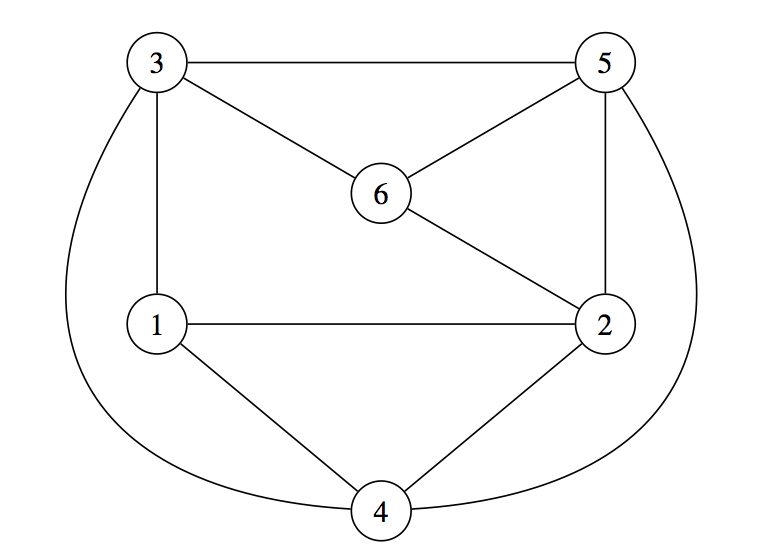
\includegraphics[width=0.8\linewidth]{fig/graph.png}
  \caption{グラフ彩色問題の例}
  \label{fig:graph}
\end{figure}
%%%%%%%%%%%%%%%%%%%%%%%%%%%%%%%%%
\lstinputlisting[float=t,caption={%
グラフ彩色問題の論理プログラム (\code{color.lp})},%
captionpos=b,frame=single,label=code:color.lp,%
numbers=left,%
breaklines=true,%
columns=fullflexible,keepspaces=true,%
basicstyle=\ttfamily\scriptsize]{code/color.lp}
%%%%%%%%%%%%%%%%%%%%%%%%%%%%%%%%%
\lstinputlisting[float=t,caption={%
\code{color.lp}に対する{\clingo}の実行例},%
captionpos=b,frame=single,label=code:color.log,%
numbers=none,%
breaklines=true,%
columns=fullflexible,keepspaces=true,%
basicstyle=\ttfamily\scriptsize]{code/color.log}
%%%%%%%%%%%%%%%%%%%%%%%%%%%%%%%%%

解集合プログラミングを用いた問題解法プロセスは,3つのステップからなる.
まず最初に,解きたい問題を論理プログラムとして表現する.
つぎに,ASP システムを用いて,論理プログラムの解集合を計算する.
最後に,解集合を解釈して元の問題の解を得る.
%
ここでは,グラフ彩色問題を例として,各ステップ毎に解法プロセスを説明する.
ASP システムとしては{\clingo}を用いる.
以降で示す論理プログラムのソースコードはすべて{\gringo}言語で書かれて
おり,表記上の対応については表~\ref{tbl:map}の通りである.

グラフ彩色問題とは,辺で結ばれたノードが同じ色にならないように,各ノー
ドを塗り分ける問題である.
例として,図~\ref{fig:graph}のグラフを赤(\code{r}),青(\code{b}),緑
(\code{g})の3色で塗り分ける問題を考える.
この問題を表す論理プログラムをコード~\ref{code:color.lp}に示す.

2〜4行目は,ノード(\code{node})と辺(\code{edge})をファクトとし
て書くことによって,図~\ref{fig:graph}のグラフを表している.
ピリオド(``\code{.}'')はルールの終わりを表す終端記号である.
7行目も同じく,色(\code{col})をファクトで表している.
%
10行目のルールは,個数制約を使って「各ノードは一つの色で塗られる」とい
う制約を表している.アトム\code{color(X,C)}は,ノード\code{X}が色
\code{C}で塗られることを意味する.コロン(\code{:})は条件付きリテラ
ルと呼ばれる拡張構文であり,このルールのヘッドは,
\code{1 \{ color(X,r);color(X,b);color(X,g) \} 1}のように展開される.
11行目のルールは,一貫性制約を使って「辺で結ばれたノード(\code{X}と
\code{Y})は,同じ色(\code{C})で塗られない」という制約を表している.

ASP システムは解集合を計算して出力する.
コード~\ref{code:color.log}に{\clingo}の実行例を示す.
この出力から,ノード1と5は緑,ノード4と6は赤,ノード2と3は青に塗り分け
られることがわかる.


% この章では,前章で挙げた諸問題を解くために利用した
% 解集合プログラミング(Answer Ser Programming; ASP
% \cite{%
%   Hayama17,%
%   Inoue08}
% )
% について,主にその言語とASPシステムについて解説する.
% 解集合プログラミングは,
% 非単調論理プログラミングが制約プログラミング(Constraint Programming; CP)の概念と融合した
% 論理プログラミングの枠組みである.\cite{Inoue08}
% そして,その記述言語は,一階論理に基づく知識表現言語の一種であり,一般拡張選言プログラム(GEDP)かそのサブクラスをベースとしているが,
% 本論文では簡単のため,GEDPのサブクラスである\textbf{標準論理プログラム}(Normal Logic Program; NLP)を説明する.

% NLPは次の形式のルールの集合である.\\
% \begin{equation}
%   \label{nlp:rule}
% l_1 ~\mcode{:-} ~l_2, ~..., ~l_m, ~not ~l_{m+1}, ~..., ~not ~l_{n}.
% \end{equation}
% 上記(\ref{nlp:rule})において,$0 \leq m \leq n$であり,
% $l_i$は正リテラル(アトム),$not$は\textbf{デフォルトの否定}\cite{Sakama10},”$,$”は連言である.
% ”$\mcode{:-}$”について,左辺が\textbf{ヘッド},右辺が\textbf{ボディ}と呼ばれ,
% ルール(\ref{nlp:rule})の直感的な意味は,
% 『$l_2, ~..., ~l_m$が全て成り立ち,$l_{m+1}, ~..., ~l_{n}$が全て成り立たないならば,$l_1$が成り立つ』
% である.

% (\ref{nlp:rule})で表されるルールの内,以下のようにボディが空のものは\textbf{ファクト}と呼ばれ,
% ”$\mcode{:-}$”を省略することができる.
% ファクト(\ref{nlp:fact}),(\ref{nlp:fact2})はどちらも『$l_1$が成り立つ』という事実を示す.
% \begin{eqnarray}
%   \label{nlp:fact}
%    l_1 ~&\mcode{:-}. \\
%   \label{nlp:fact2}
%    l_1.&
% \end{eqnarray}

% 一方で,以下のようにヘッドが空であるルールは\textbf{一貫性制約}と呼ばれる.
% \begin{equation}
%   \mcode{:-} ~l_2, ~..., ~l_m, ~not ~l_{m+1}, ~..., ~not ~l_{n}.
% \end{equation}
% 例えば,一貫性制約(\ref{nlp:cons})は『$b$が成り立ってはならない』という制約を,
% (\ref{nlp:cons2})は『$b$が成り立たなければならない』という制約をそれぞれ示す.
% \begin{eqnarray}
%   \label{nlp:cons}
%    \mcode{:-}& ~b.\\
%   \label{nlp:cons2}
%    \mcode{:-}& ~not ~b.
% \end{eqnarray}

% さらに,本研究にて用いたものを含む最新のASP言語には,
% \textbf{アグリゲート}という表記法が実装されており,組み合わせ問題を簡潔に記述することができる.
% 例えば,\textbf{選択子}(\ref{choice})を使うことで,集合$\{l_1, ~..., ~l_k\}$の任意の部分集合を
% 後述の\textbf{解集合}に含むことを指定できる.さらに,以下(\ref{numcon})のようにこの選択子の左右に数字を指定することで,
% 選択子が選択可能なリテラル個数の上下限を指定することができる.$ln$が下限で,$mn$が上限である.
% \begin{eqnarray}
%   \label{choice}
%   \{l_1, ~.&.&., ~l_k\} \\
%   \label{numcon}
%   ln ~\{l_1, ~.&.&., ~l_k\} ~mn
% \end{eqnarray}

% また,先述の最短ハミルトン路・閉路問題のような組合せ最適化問題の実装時には,
% 最小化関数$\#minimize$や最大化関数$\#maximize$を用いることができる.
% さらに,先述の制約付きハミルトン路問題を解くにあたり必要であった目的関数値の制約は,
% \textbf{重み付き個数制約}”$\#sum\{w_1:l_1; ~...;~w_k:l_k\} < c$”を用いて実装した.
% これは,$l_i$に対応する重み$w_i$について,値が真となるリテラル$l_i$の重みの総和がcより小さいという制約である.

% ASPシステムは,与えられたGEDPやNLPから,そこに書かれた全てのルールを満たすように,安定モデル意味論
% \cite{%
%   Inoue08,%
%   Gelfond88%
% }
% に基づく解集合を計算するシステムである.本研究では,ASPシステム \clingo を使用した.
%  \clingo は グラウンダー \gringo とASPソルバー \clasp から構成され,
%  \gringo は \clingo に与えられた一階ASPプログラムを命題ASPプログラムに変換する\textbf{基礎化}
% を行った後に基礎化後のプログラムを \clasp に渡し,その後, \clasp が解集合を算出する.
% \newpage
% %% \[
% %% %\tabcolsep = 2mm
% %% \begin{array}{c|c|c|c}
% %%        X                   & \reduct{P}{X}  & 
% %% \reduct{P}{X}\textrm{の最小モデル}  & X\textrm{は}P\textrm{の解集合?}\\\hline
% %% \{\phantom{p         ,q}\} & \{p\leftarrow,\quad q\leftarrow\}             & \{p,q\}    
% %% &  \times \\\hline
% %% \{         p\phantom{,q}\} & \{p\leftarrow\phantom{\quad q\leftarrow}\}    & \{p\}      
% %% & \circ \\\hline
% %% \{\phantom{p,}        q \} & \{\phantom{p\leftarrow,\quad} q \leftarrow\}  & \{q\}      
% %% & \circ \\\hline
% %% \{         p         ,q \} & \{\phantom{p\leftarrow,\quad q\leftarrow}\}   & \emptyset  
% %% & \times \\\hline
% %% \end{array}
% %% \]

% %% %%%%%%%%%%%%%%%%%%%%%%%%%%%%%%%%%
% %% \begin{table}[tb]
% %%   \centering
% %%   \begin{tabular}{l|*{4}{p{1cm}}}
% %%     論理プログラム &   $\leftarrow$ & $,$        & $;$        & $\sim$       \\\hline
% %%     ソースコード   &   \texttt{:-}  & \texttt{,} & \texttt{;} & \texttt{not}
% %%   \end{tabular}
% %%   \caption{論理プログラムとソースコードの対応}
% %%   \label{tbl:map}
% %% \end{table}
% %% %%%%%%%%%%%%%%%%%%%%%%%%%%%%%%%%%
% %% \begin{figure}[tb]
% %%   \centering
% %%   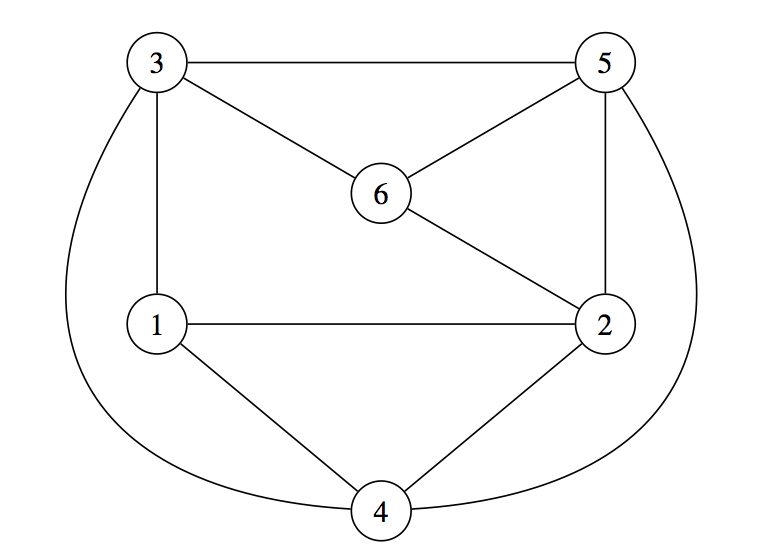
\includegraphics[width=0.6\linewidth]{fig/graph.png}
% %%   \caption{グラフ}
% %%   \label{fig:graph}
% %% \end{figure}
% %% %%%%%%%%%%%%%%%%%%%%%%%%%%%%%%%%%
% %% \lstinputlisting[float=t,caption={%
% %% グラフ彩色問題の論理プログラム (\code{color.lp})},%
% %% captionpos=b,frame=single,label=code:color.lp,%
% %% numbers=left,%
% %% breaklines=true,%
% %% columns=fullflexible,keepspaces=true,%
% %% basicstyle=\ttfamily\scriptsize]{code/color.lp}
% %% %%%%%%%%%%%%%%%%%%%%%%%%%%%%%%%%%
% %% \lstinputlisting[float=t,caption={%
% %% \code{color.lp}に対する{\clingo}の実行例},%
% %% captionpos=b,frame=single,label=code:color.log,%
% %% numbers=none,%
% %% breaklines=true,%
% %% columns=fullflexible,keepspaces=true,%
% %% basicstyle=\ttfamily\scriptsize]{code/color.log}
% %% %%%%%%%%%%%%%%%%%%%%%%%%%%%%%%%%%

%%% Local Variables:
%%% mode: japanese-latex
%%% TeX-master: "paper"
%%% End:
